\documentclass{article}
% Language setting
% Replace `english' with e.g. `spanish' to change the document language
\usepackage[english]{babel}


% Set page size and margins
% Replace `letterpaper' with `a4paper' for UK/EU standard size
\usepackage[a4paper,top=2cm,bottom=2cm,left=3cm,right=3cm,marginparwidth=1.75cm]{geometry}

% Useful packages
\usepackage[utf8]{inputenc}
\usepackage{fontspec} 
\setmonofont{Fira Code}[Scale=0.9]

\usepackage{array}
\usepackage[most]{tcolorbox} % for inline code
\usepackage{amsmath}
\usepackage{graphicx}
\usepackage{subfigure}
\usepackage[colorlinks=true, allcolors=blue]{hyperref}
\usepackage{authblk}
\usepackage{amssymb}
\usepackage{listings}
\usepackage{color}
\usepackage{xcolor}
\usepackage{float}
\usepackage{biblatex} %Imports biblatex package
\addbibresource{references.bib} %Import the bibliography file
\usepackage{wrapfig}
\usepackage{booktabs}
\usepackage{longtable}

\renewcommand{\floatpagefraction}{0.1}
\renewcommand{\textfraction}{0}

\definecolor{dkgreen}{rgb}{0,0.6,0}
\definecolor{gray}{rgb}{0.5,0.5,0.5}
\definecolor{mauve}{rgb}{0.58,0,0.82}
\definecolor{lightgray}{gray}{0.9}

\lstdefinestyle{pythonstyle}{
  language=Python,
  frame=tb,
  aboveskip=3mm,
  belowskip=3mm,
  showstringspaces=false,
  columns=flexible,
  basicstyle={\ttfamily\small},
  numbers=left,
  numberstyle=\tiny\color{gray},
  keywordstyle=\color{blue},
  commentstyle=\color{green!50!black},
  stringstyle=\color{red!70!black},
  breaklines=true,
  breakatwhitespace=true,
  tabsize=4,
  captionpos=b,
  morekeywords={self, cls, __init__, None},
}

\lstdefinestyle{pseudocode}{frame=tb,
  language=Python,
  aboveskip=3mm,
  belowskip=3mm,
  showstringspaces=false,
  columns=flexible,
  basicstyle={\small\ttfamily},
  numbers=left,
  numberstyle=\tiny\color{gray},
  keywordstyle=\color{blue},
  commentstyle=\color{dkgreen},
  stringstyle=\color{mauve},
  breaklines=true,
  breakatwhitespace=true,
  tabsize=3
}

\lstdefinestyle{input}{frame=none,
  aboveskip=3mm,
  belowskip=3mm,
  showstringspaces=false,
  columns=flexible,
  basicstyle={\small\ttfamily},
  numbers=none,
  numberstyle=\tiny\color{gray},
  keywordstyle=\color{blue},
  commentstyle=\color{dkgreen},
  stringstyle=\color{mauve},
  breaklines=true,
  breakatwhitespace=true,
  tabsize=3,
  captionpos=b,
}

% inline code display
\newtcbox{\inlinecode}{
  nobeforeafter, 
  colback=lightgray, 
  colframe=white, 
  boxrule=0pt, 
  arc=1mm, 
  left=0pt, right=0pt, top=0pt, bottom=0pt,
  on line,
  fontupper=\scriptsize\ttfamily
}


% make title
\title{
\includegraphics[scale=0.2]{Cam_logo_bw.png}\\
\vspace{0.5cm}
C1 Research Computing Coursework
}
\author{xl628}
\affil{Department of Physics, University of Cambridge}

\begin{document}

\maketitle

\vspace{1cm}
\noindent
\textbf{Document Statistics:} \\
Words in text: 2316 \\
Words in headers: 79 \\
Words outside text (captions, etc.): 29 \\
Number of headers: 33 \\
Number of floats/tables/figures: 6 \\
Number of math inlines: 24 \\
Number of math displayed: 13

%----------------------------------------------------------------------------------
\section{Introduction}
Automatic differentiation is a fundamental tool for optimizing learning algorithms in deep neural networks. Forward-mode automatic differentiation using dual number is efficient in scenarios with few input variables and many output variables. This report presents the development of a dual-number-based automatic differentiation package, \texttt{dual\_autodiff}, along with its Cythonized counterpart, \texttt{dual\_autodiff\_x}. 

%----------------------------------------------------------------------------------
\section{Project Structure and Configuration}

\subsection{Project Structure}

The project directory is organized as follows:

\begin{verbatim}
xl628/
├── docs/
│   ├── Makefile
│   ├── build/
│   ├── make.bat
│   └── source/
├── dual_autodiff/
│   ├── dual_autodiff/
│   ├── pyproject.toml
│   └── tests/
├── dual_autodiff_x/
│   ├── dual_autodiff_x/
│   ├── pyproject.toml
│   ├── setup.py
│   └── wheelhouse/
├── notebooks/
├── report/
├── README.md
├── .gitignore
└── requirements.txt
\end{verbatim}

The main contents are as follows:

\begin{itemize}
    \item \texttt{docs/}: Contains the Sphinx documentation for the project.
    \item \texttt{dual\_autodiff/}: Contains the implementation of the dual-number automatic differentiation package.
    \begin{itemize}
        \item \texttt{dual\_autodiff/dual\_autodiff/\_\_init\_\_.py}: Initializes the package, imports the \texttt{Dual} class, and displays the package version.
        \item \texttt{dual\_autodiff/dual\_autodiff/dual.py}: Implements the base class \texttt{Dual} and the associated methods required for automatic differentiation.
        \item \texttt{dual\_autodiff/pyproject.toml}: Configuration file defining package dependencies and the build system.
    \end{itemize}
    \item \texttt{dual\_autodiff\_x/}: Contains the Cythonized version of the \texttt{dual\_autodiff} package.
    \item \texttt{notebooks/}: Includes example notebooks demonstrating the functionality of the project. Examples include differentiating specific functions and performance comparisons between \texttt{dual\_autodiff} and \texttt{dual\_autodiff\_x}.
    \item \texttt{report/}: Holds reports and related files.
    \item \texttt{README.md}: The project's main README file.
    \item \texttt{requirements.txt}: Lists project dependencies.
    \item \texttt{.gitignore}: Specifies files and directories to be excluded from version control.
\end{itemize}

\subsection{Configuration}
\texttt{pyproject.toml} is a configuration file used by packaging tools \cite{python_packaging_pyproject_toml}. There are three possible TOML tables in the configuration file: \texttt{build-system}, \texttt{project}, and \texttt{tool}.

\begin{itemize}
    \item \texttt{build-system}: Specifies the build backend and its required dependencies.
    \begin{itemize}
        \item In this project, the build backend is \texttt{setuptools.build\_meta}, and the build dependencies include \texttt{setuptools} and \texttt{wheel}.
    \end{itemize}
    \item \texttt{project}: Contains project metadata such as the name, version, description, authors, and dependencies.
    \item \texttt{tool}: Holds tool-specific configuration subtables, which are defined by the corresponding tools.
    \begin{itemize}
        \item For example, we configure \texttt{pytest} to run tests under the \texttt{[tool.pytest.ini\_options]} table.
    \end{itemize}
\end{itemize}


\section{Implementation of Dual Number Automatic Differentiation}

\subsection{Mathematical Background\cite{automatic_differentiation_wikipedia}}

\subsubsection*{Dual Numbers}

A dual number is defined as an ordered pair $(a, b)$, typically written as $a + b\epsilon$, where:

\begin{itemize}
    \item $a, b \in \mathbb{R}$ (the real numbers)
    \item $\epsilon$ is the dual unit with the property $\epsilon^2 = 0$
\end{itemize}

\subsubsection*{Basic Operations}

The algebraic structure of dual numbers defines the following basic operations:

\begin{enumerate}
    \item \textbf{Addition and Subtraction}: 
    \[
    (a + b\epsilon) \pm (c + d\epsilon) = (a \pm c) + (b \pm d)\epsilon
    \]
    
    \item \textbf{Multiplication}: 
    \[
    (a + b\epsilon)(c + d\epsilon) = ac + (bc + ad)\epsilon \quad \text{(since $\epsilon^2 = 0$)}
    \]

    \item \textbf{Division} (for $c \neq 0$): 
    \[
    \frac{a + b\epsilon}{c + d\epsilon} = \frac{a}{c} + \frac{bc - ad}{c^2}\epsilon
    \]

    \item \textbf{Power Rules}: 
    \[
    (a + b\epsilon)^n = a^n + nba^{n-1}\epsilon
    \]
\end{enumerate}

\subsubsection*{Automatic Differentiation Theory}

The key insight of forward-mode automatic differentiation is that dual numbers naturally encode derivative information through the formula. Given $x = a + b\epsilon$, and a function $f(x)$, we have:

\[
f(x) = f(a + b\epsilon) = f(a) + f'(a)b\epsilon
\]

And so, $f'(a)$ can be extracted from the coefficient of the $\epsilon$ term in the dual number $f(a + b\epsilon)$.

This formula emerges from the Taylor series expansion and the property of $\epsilon$:

\[
f(a + b\epsilon) = f(a) + f'(a)(b\epsilon) + \frac{f''(a)}{2!}(b\epsilon)^2 + \cdots = f(a) + f'(a)b\epsilon
\]

The chain rule emerges naturally from dual number arithmetic. For composite functions like $h(x) = f(g(x))$:

\[
h(a + b\epsilon) = f(g(a + b\epsilon)) = f(g(a) + g'(a)b\epsilon) = f(g(a)) + f'(g(a))g'(a)b\epsilon
\]

where we get $f'(g(a))g'(a)$ as the derivative of the composite function.

\subsubsection*{Elementary Functions}

Using the Taylor series expansion and the property of $\epsilon$, we can derive the following formulas for the elementary functions:

\begin{enumerate}
    \item \textbf{Exponential}: 
    \[
    \exp(a + b\epsilon) = e^a + be^a\epsilon
    \]

    \item \textbf{Logarithm} (for $a > 0$): 
    \[
    \log(a + b\epsilon) = \log(a) + \frac{b}{a}\epsilon
    \]

    \item \textbf{Trigonometric Functions}: 
    \begin{itemize}
        \item $\sin(a + b\epsilon) = \sin(a) + b\cos(a)\epsilon$
        \item $\cos(a + b\epsilon) = \cos(a) - b\sin(a)\epsilon$
        \item $\tan(a + b\epsilon) = \tan(a) + \frac{b}{\cos^2(a)}\epsilon$
    \end{itemize}
\end{enumerate}

\subsection{Implementation}

The \texttt{dual.py} file contains the implementation of the base class \texttt{Dual} along with the necessary methods for automatic differentiation. The class supports the following functionalities:

\begin{itemize}
    \item \textbf{Basic Arithmetic Operations}
    \begin{itemize}
        \item Addition: \texttt{\_\_add\_\_}, \texttt{\_\_radd\_\_}
        \item Subtraction: \texttt{\_\_sub\_\_}, \texttt{\_\_rsub\_\_}
        \item Multiplication: \texttt{\_\_mul\_\_}, \texttt{\_\_rmul\_\_}
        \item Division: \texttt{\_\_truediv\_\_}
        \item Exponentiation: \texttt{\_\_pow\_\_}
    \end{itemize}
    
    \item \textbf{Elementary Functions:}
    \begin{itemize}
        \item Exponential: \texttt{exp}
        \item Logarithm: \texttt{log}
        \item Trigonometric: \texttt{sin}, \texttt{cos}, \texttt{tan}
    \end{itemize}
    
    \item \textbf{Support Methods:}
    \begin{itemize}
        \item \texttt{\_\_init\_\_}: Initializes a dual number with real and dual components. By default, the dual part is set to 1.0 to facilitate derivative computations.
        \item \texttt{\_\_repr\_\_} and \texttt{\_\_str\_\_}: Provide string representations in the format \texttt{Dual(real=x, dual=y)}.
        \item \texttt{\_\_neg\_\_}: Implements unary negation as \( -(a + b\epsilon) = -a + (-b)\epsilon \).
    \end{itemize}
\end{itemize}

Each method includes proper type checking and error handling, raising appropriate exceptions for invalid operations. The implementation supports operations between dual numbers, and also supports some operations between dual numbers and regular numbers (float/int).

Below are basic examples demonstrating the functionality:
\begin{lstlisting}[style=pythonstyle]
# basic operations
x = Dual(2, 1)
y = Dual(3, 1)
print(x + y)

# trigonometric functions
print(Dual(2, 1).sin())

# alternative way to use the method
x = Dual(2, 1)
print(Dual.sin(x))
\end{lstlisting}
The corresponding output is:
\begin{lstlisting}[style=input]
Dual(real=5, dual=2)
Dual(real=0.9092974268256817, dual=-0.4161468365471424)
Dual(real=0.9092974268256817, dual=-0.4161468365471424)
\end{lstlisting}

\subsection{Example: Differentiating a Function}

The \texttt{notebooks/differentiate\_function.ipynb} notebook provides a practical example of using the \texttt{Dual} class to compute the derivative of a function:
\[
f(x) = \log(\sin(x)) + x^2 \cos(x),
\]
with the analytical derivative:
\[
f'(x) = \frac{\cos(x)}{\sin(x)} + 2x \cos(x) - x^2 \sin(x).
\]

In this example, we compare three derivative computation methods: analytical differentiation, numerical differentiation, and automatic differentiation using the \texttt{Dual} class. The numerical derivative is calculated using the central difference formula:
\[
f'(x) = \frac{f(x+h) - f(x-h)}{2h},
\]
We measure the accuracy of the method using relative error and evaluate the derivatives at $x=1.5$. The results are illustrated in Fig. \ref{fig:error}.

\begin{figure}[!htbp]
\centering
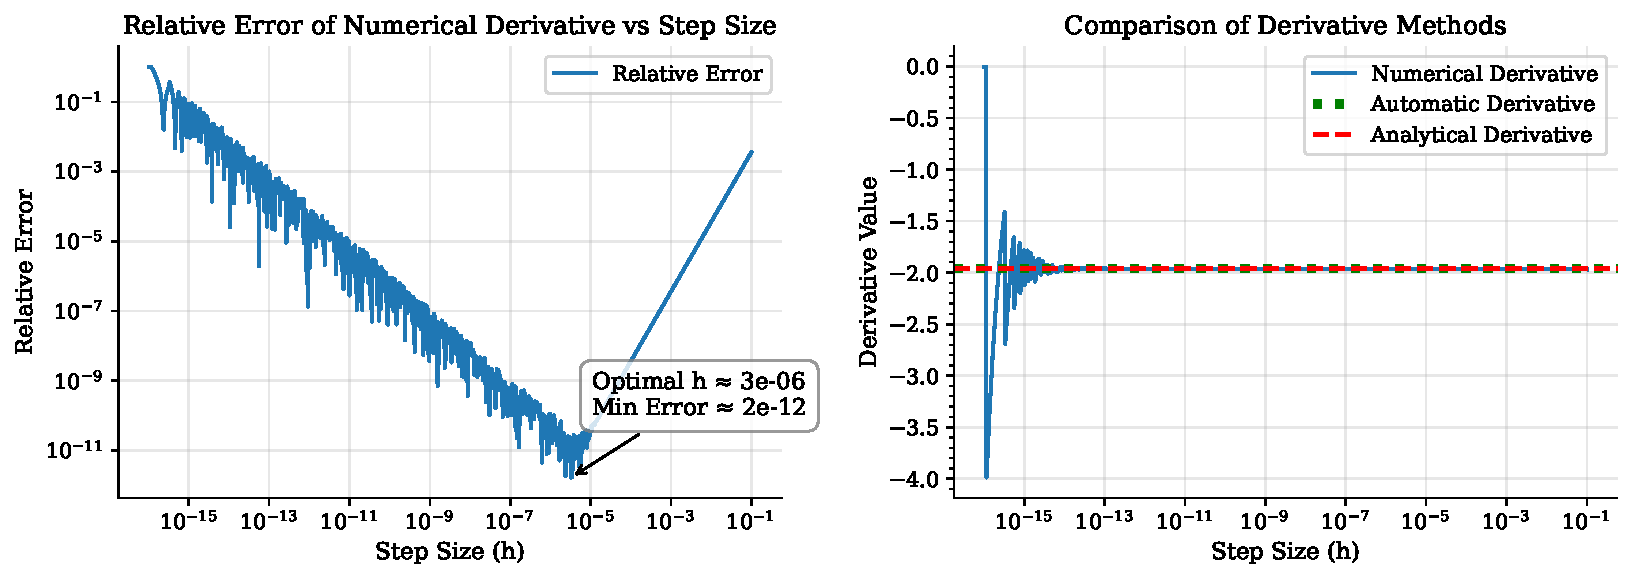
\includegraphics[width=0.94\textwidth]{./images/derivative_comparison.pdf}
\caption{Comparison of Derivative Methods}
\label{fig:error}
\end{figure}



Automatic differentiation using \texttt{Dual} class provides a more accurate result than numerical differentiation, with significantly smaller relative errors:

\begin{lstlisting}[style=input]
Analytical derivative at x=1.5: -1.9612372705533612
Value at x=1.5: 0.15665054756073515
AutoDiff derivative at x=1.5: -1.9612372705533612
AutoDiff relative error: 0.0
\end{lstlisting}

When reducing the step size, the error in the numerical derivative does not decrease as expected but instead oscillates and increases. This instability suggests that numerical differentiation is sensitive to step size and may fail for singular or non-differentiable functions. Conversely, increasing the step size beyond a certain point also results in larger errors due to loss of precision.

From the figure, the optimal step size for this function is approximately $3 \times 10^{-6}$.

\section{Package Development}

\subsection{Development Installation}

To install the package for development, navigate to the root directory (\texttt{xl628/dual\_autodiff/}) and run the following command:

\begin{lstlisting}[style=input]
pip install -e . 
\end{lstlisting}

This will install the package in editable mode.

To verify the installation, open a Python shell, import the \texttt{Dual} class, and create a \texttt{Dual} object:

\begin{lstlisting}[style=pythonstyle]
>>> from dual_autodiff.dual_autodiff.dual import Dual
>>> x = Dual(2.0, 1.0)
>>> print(x)
Dual(real=2.0, dual=1.0)
\end{lstlisting}

If the installation is successful, no errors should occur.

\subsection{Testing Strategy}

The test suite is implemented using \texttt{pytest}. Before running the tests, ensure that all development requirements, including \texttt{pytest} and \texttt{pytest-cov}, are installed. Run the following command at the root directory (e.g., \texttt{xl628/}):

\begin{lstlisting}[style=input]
pip install -r requirements.txt
\end{lstlisting}

To execute the tests, use:

\begin{lstlisting}[style=input]
pytest 
\end{lstlisting}

Run this command from the root directory of the package, i.e., \texttt{xl628/dual\_autodiff/}.

The test suite includes:

\begin{itemize} 
    \item Basic initialization and string representation checks \item Arithmetic operations, including proper error handling \item Verification of elementary functions (e.g., trigonometric, exponential, logarithmic) 
    \item Validation of chain rule implementation 
\end{itemize}

Both the real and dual parts of calculations are tested for accuracy. Numerical results are validated using \texttt{pytest.approx()} with a relative tolerance of 1e-5. For details, refer to the source code in \texttt{xl628/dual\_autodiff/tests/test\_dual.py}.

To ensure conciseness and maintainability, we use \texttt{pytest}'s \texttt{parametrize} decorator to test multiple cases efficiently.

Test coverage reports are automatically generated using \texttt{pytest-cov} whenever the tests are executed.

All tests passed in my experiment.

\section{Documentation}

The documentation is built using \texttt{Sphinx} and \texttt{nbsphinx} with the \texttt{readthedocs} theme. It provides comprehensive details, including:

\begin{itemize} 
    \item Installation instructions 
    \item Usage examples 
    \item API reference 
    \item A mathematical introduction to dual numbers and automatic differentiation 
\end{itemize}

\texttt{Sphinx} is a powerful tool for generating structured and beautiful documentation using reStructuredText as its markup language \cite{sphinx_pypi}. The \texttt{nbsphinx} extension allows integration of Jupyter notebooks into the documentation \cite{nbsphinx_docs}.

\subsection{Building the Documentation}

To build the documentation, install the development requirements and run the following commands from the \texttt{docs} directory:

\begin{lstlisting}[style=input]
pip install -r requirements.txt
cd docs
make html
\end{lstlisting}

The generated HTML documentation will be available in the \texttt{docs/build/html} directory. To clean the build, use:

\begin{lstlisting}[style=input] 
make clean 
\end{lstlisting}

\subsection{Documentation Examples}

The \textit{Getting Started} section includes basic examples demonstrating the use of the package for derivatives, mathematical operations, and elementary functions. More advanced examples are provided in the \textit{Applications} section, where the \texttt{Dual} class is used to compute partial derivatives and gradients.

The gradient example serves as a solid foundation for further applications such as optimization, neural networks, and other numerical techniques.

\section{Cythonization and Performance Analysis}

\subsection{Cythonized Package}

The \texttt{dual\_autodiff\_x} package is the cythonized version of \texttt{dual\_autodiff}. It is built using the \texttt{Cython} extension. \cite{cython_org}\cite{cython_docs_quickstart}

\textbf{Cython} is a programming language designed to simplify the creation of C extensions for Python. It serves as a superset of Python, offering features like optional static type declarations and seamless integration with external C libraries.

Cython translates Python-like source code into optimized C/C++ code, which is then compiled into Python extension modules. This process results in significantly faster execution while maintaining Python's high-level functionality and developer-friendly syntax.

Cython is widely used in performance-critical research computing libraries, such as \texttt{NumPy}, \texttt{SciPy}, \texttt{Pandas}, and \texttt{scikit-learn} \cite{researchcomputing_notebook}. The key performance improvements stem from:

\begin{itemize} 
    \item \textbf{Static Typing:} Variables can be explicitly declared with C types to eliminate Python's dynamic type overhead. 
    \item \textbf{Reduced Overhead:} Cython avoids Python's interpreter overhead, enabling faster function execution. 
    \item \textbf{Compiler Optimizations:} Cython leverages C-level optimizations for loops and arithmetic operations. 
\end{itemize}

In the \texttt{dual\_autodiff\_x} package, Cython source files (\texttt{.pyx}) are compiled to generate intermediate files (\texttt{.c} and \texttt{.cpp}) and shared object files (\texttt{.so}). Developers can optimize the \texttt{.pyx} files further by incorporating static type declarations and C libraries.

\subsection{Performance Analysis}

Performance comparisons between the \texttt{dual\_autodiff} (Python version) and \texttt{dual\_autodiff\_x} (Cython version) are conducted in the \texttt{notebooks/performance\_comparison.ipynb} notebook. The evaluation considers multiple aspects, including:

\begin{itemize} \item Basic operations \item Mathematical functions \item Scaling behavior \item Memory usage \item Real-world applications \end{itemize}

The summarized results are presented in Table \ref{tab:overall_performance_summary}. Overall, the cythonized version demonstrates substantial improvements in both speed and memory efficiency.

\begin{longtable}{ll}
\caption{Overall Performance Summary.}\label{tab:overall_performance_summary}\\
\toprule
\textbf{Category} & \textbf{Details} \\
\midrule
\endfirsthead
\toprule
\textbf{Category} & \textbf{Details} \\
\midrule
\endhead
\bottomrule
\endfoot
\multicolumn{2}{l}{\textbf{1. Basic Operations:}} \\
Average speedup & 1.91x \\
Best performing & Power (2.44x) \\
Average improvement & 46.7\% \\
\midrule
\multicolumn{2}{l}{\textbf{2. Mathematical Functions:}} \\
Average speedup & 2.07x \\
Best performing & Logarithm (2.23x) \\
Average improvement & 51.7\% \\
\midrule
\multicolumn{2}{l}{\textbf{3. Scaling Analysis:}} \\
Maximum speedup & 3.11x at chain length 100 \\
Speedup trend & Increases with chain length \\
\midrule
\multicolumn{2}{l}{\textbf{4. Memory Usage:}} \\
Average memory ratio (Python/Cython) & 1.87 \\
Maximum memory savings & 50.5\% \\
\midrule
\multicolumn{2}{l}{\textbf{5. Real-world Applications:}} \\
Average speedup & 2.31x \\
Best performing & Gradient Computation (2.61x) \\
Average improvement & 56.3\% \\
\midrule
\multicolumn{2}{l}{\textbf{Overall Assessment:}} \\
Global average speedup & 2.33x \\
Performance improvement range & 1.7x - 3.1x \\
\bottomrule
\end{longtable}


\subsubsection*{Basic Operations}

We evaluate the performance of basic operations, including creation, addition, multiplication, division, and exponentiation. The \texttt{measure\_time} function from \texttt{performance\_benchmark.py} is used with \texttt{n\_runs=1,000,000} to collect execution time statistics.

The results are summarized in Fig. \ref{fig:bo}.

\begin{figure}[!htbp]
\centering
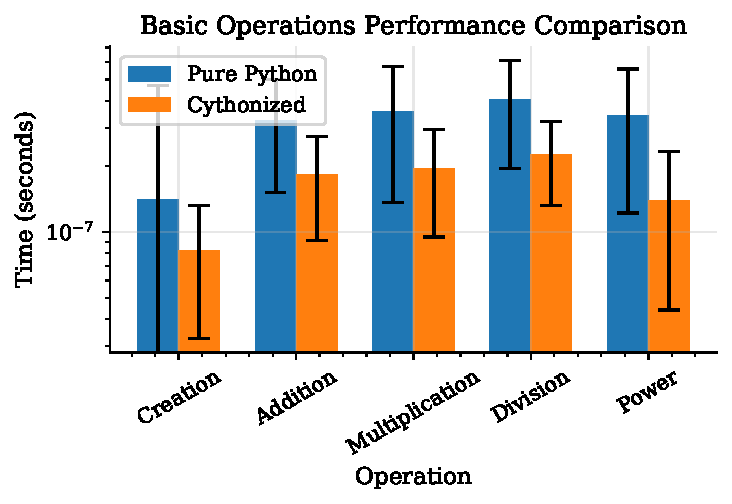
\includegraphics[width=0.47\textwidth]{./images/basic_ops_performance.pdf}
\caption{Performance of Basic Operations}
\label{fig:bo}
\end{figure}

The results show that the cythonized version significantly outperforms the Python version, achieving an average speedup of 1.91x. Among all operations, the power operation demonstrates the greatest improvement, with a speedup of 2.44x. This is likely because, unlike other operations, the implementation of the power function explicitly accepts \texttt{int} or \texttt{float} types but not \texttt{Dual} types. As a result, static typing using \texttt{double} could be applied in the Cython implementation, allowing the compiler to determine variable types at compile time, thereby eliminating runtime checks and improving computational efficiency.

\subsubsection*{Mathematical Functions}

We also analyze the performance of mathematical functions, including the exponential, sine, cosine, and logarithm functions. Using the same \texttt{measure\_time} function with \texttt{n\_runs=1,000,000}, we collect execution time statistics.

The results are shown in Fig. \ref{fig:mf}.
\newpage
\begin{figure}[!htbp]
\centering
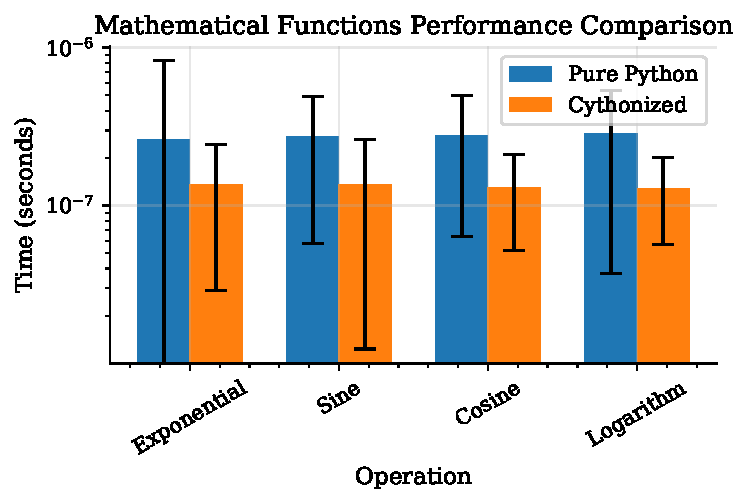
\includegraphics[width=0.47\textwidth]{./images/math_funcs_performance.pdf}
\caption{Performance of Mathematical Functions}
\label{fig:mf}
\end{figure}

The cythonized version shows strong performance improvements, with an average speedup of 2.07x. Among all functions, the logarithm function achieves the highest speedup at 2.23x. In addition to static typing, these improvement are due to the use of the C math library, which optimizes the computation of these mathematical functions.



\subsubsection*{Scaling Analysis}

To assess scaling performance, we analyze computations with increasing chain lengths. This is particularly relevant in neural network backpropagation, where chain derivatives are common. For this experiment, \texttt{n\_runs=100,000} is used to collect execution time statistics.

In this experiment, we construct a chain of functions based on $f(x) = \sin(\exp(\log(x)))$, where the chain is defined as 
$f(f(...f(x)...))$. We measure the performance for varying chain lengths.

\begin{lstlisting}[style=pythonstyle]
def chain(x):
    result = impl.Dual(x, 1.0)
    for _ in range(n):
        result = result.sin().exp().log()
    return result
\end{lstlisting}

The chain lengths tested are \texttt{[1, 2, 5, 10, 20, 50, 100]}.

The results are presented in Fig. \ref{fig:sa}.

\begin{figure}[!htbp]
\centering
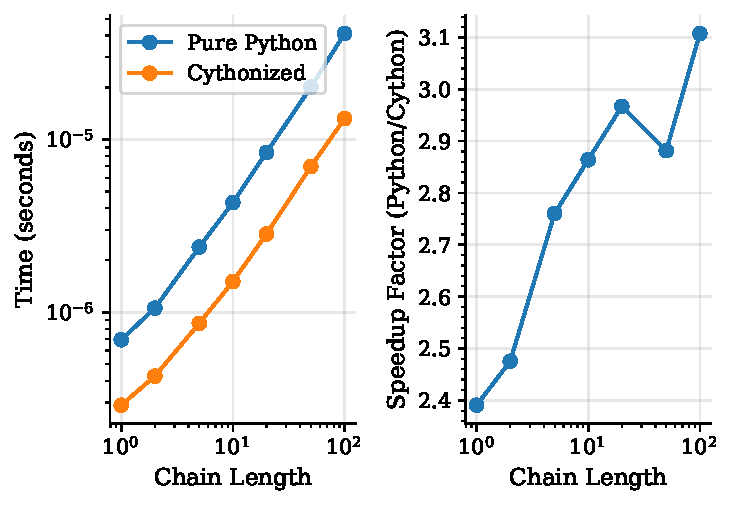
\includegraphics[width=0.47\textwidth]{./images/scaling_analysis.pdf}
\caption{Scaling Performance with Increasing Chain Length}
\label{fig:sa}
\end{figure}

The analysis reveals that the speedup increases with chain length, reaching a maximum of 3.11x at the longest chain. This trend suggests that the optimized implementation scales efficiently with larger inputs, likely due to reduced overhead and improved data handling at scale.

\subsubsection*{Memory Usage}

We measure memory usage by creating arrays of \texttt{Dual} objects of varying sizes. The \texttt{memory\_usage} function from \texttt{performance\_benchmark.py} is used for this purpose. The array sizes tested are:

\begin{lstlisting}[style=pythonstyle]
array_sizes = [1000000, 5000000, 10000000]

def create_array(size, impl):
    return [impl.Dual(x_val, 1.0) for _ in range(size)]
\end{lstlisting}

The results are illustrated in Fig. \ref{fig:mu}.

\begin{figure}[!htbp]
\centering
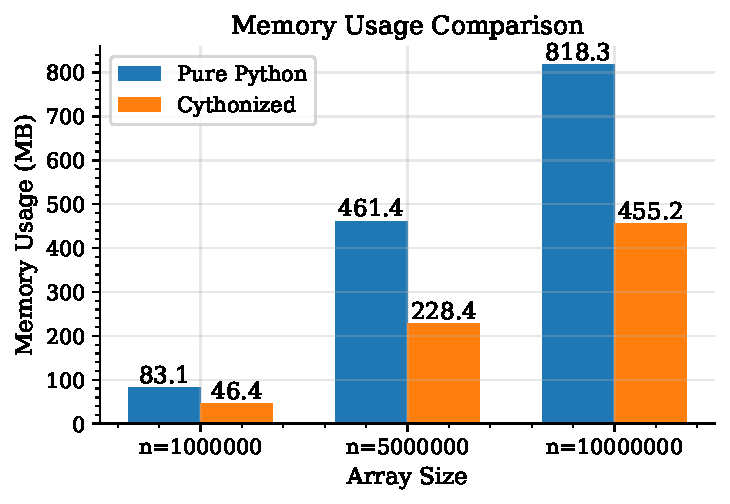
\includegraphics[width=0.47\textwidth]{./images/memory_usage.pdf}
\caption{Memory Usage for Array Creation}
\label{fig:mu}
\end{figure}

The cythonized version significantly reduces memory usage, achieving a maximum reduction of 50.5\%. This improvement can be attributed to more efficient memory management in Cython.

\subsubsection*{Applications}

To assess real-world applicability, we benchmark three scenarios where derivatives are useful:

\begin{itemize} 
\item Neural network forward propagation 
\item Gradient computation 
\item Physics simulation 
\end{itemize}

Execution times are measured using the \texttt{measure\_time} function with \texttt{n\_runs=1,000,000}. The results are shown in Fig. \ref{fig:app}:

\begin{figure}[!htbp]
\centering
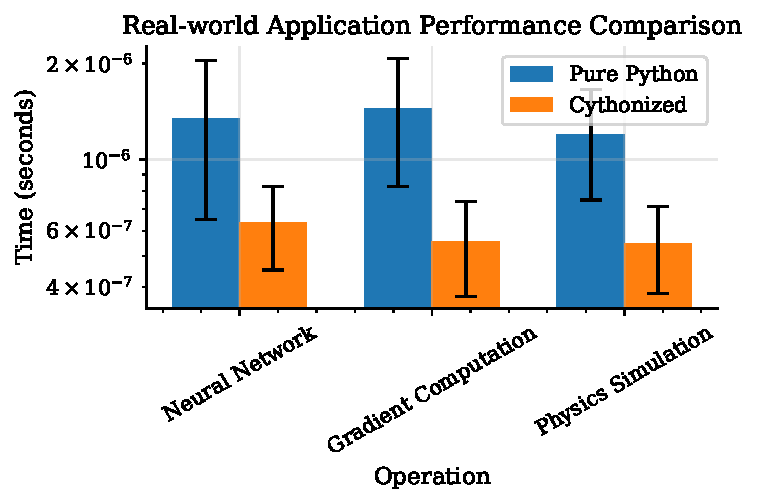
\includegraphics[width=0.47\textwidth]{./images/app_performance.pdf}
\caption{Application Performance Comparison}
\label{fig:app}
\end{figure}

The results demonstrate significant performance gains in practical applications. Gradient computation achieves the largest improvement, with a speedup of 2.61x, underscoring the advantages of the optimized Cython implementation for computationally intensive tasks.

\section{Linux Wheel Generation}

We use \texttt{cibuildwheel} to generate the wheel for the \texttt{dual\_autodiff\_x} package.

\texttt{cibuildwheel} supports building wheels for CPython and PyPy across various platforms, including manylinux, musllinux, macOS, and Windows \cite{cibuildwheel}.

\subsection{Wheel Generation}

The wheel is generated using the following command:
\[
\texttt{CIBW\_BUILD="cp311-manylinux\_x86\_64" CIBW\_ARCHS="x86\_64" cibuildwheel --platform linux}
\]
we can specify the Python version, the platform, and the architecture we want to build for.

Here:

\begin{itemize} 
    \item \texttt{cp} denotes CPython, and \texttt{311} specifies Python version 3.11. 
    \item \texttt{manylinux} indicates the manylinux platform, a standardized environment for building Linux wheels. 
    \item \texttt{x86\_64} refers to the 64-bit x86 CPU architecture. \end{itemize}

In this case, we build wheels for Python 3.10 and Python 3.11 on the manylinux platform with x86\_64 architecture. The resulting wheels are stored in the \texttt{dual\_autodiff\_x/wheelhouse} directory.

Additionally, the \texttt{setup.py} file is configured as follows:

\begin{itemize} 
    \item \texttt{package\_data} and \texttt{exclude\_package\_data} ensure that only the \texttt{.so} files are included, while the \texttt{.pyx} and \texttt{.py} source files are excluded to prevent their distribution. 
    \item \texttt{zip\_safe=False} is specified for wheel generation.
\end{itemize}

\subsection{Wheel Installation on CSD3}

To verify the generated wheel, we install it on the CSD3 server as follows:

\begin{lstlisting}[style=input]
(venv_EC1_311) [xl628@login-q-1 wheelhouse]$ pip install dual_autodiff_x-0.0.1-cp311-cp311-manylinux_2_17_x86_64.manylinux2014_x86_64.whl 
Processing ./dual_autodiff_x-0.0.1-cp311-cp311-manylinux_2_17_x86_64.manylinux2014_x86_64.whl
Installing collected packages: dual-autodiff-x
Successfully installed dual-autodiff-x-0.0.1
\end{lstlisting}

Next, we validate the installation by importing the \texttt{Dual} class and performing a basic computation:

\begin{lstlisting}[style=input]
(venv_EC1_311) [xl628@login-q-2 ~]$ python3
Python 3.11.9 (main, Sep 24 2024, 09:39:15) [GCC 8.5.0 20210514 (Red Hat 8.5.0-22)] on linux
Type "help", "copyright", "credits" or "license" for more information.
>>> import dual_autodiff_x as df
dual_autodiff_x package version: 0.0.1
>>> x = df.Dual(2, 1)
>>> sinx = x.sin()
>>> print(sinx)
Dual(real=0.9092974268256817, dual=-0.4161468365471424)
\end{lstlisting}

As demonstrated, the \texttt{Dual} class operates correctly on the CSD3 server, confirming that the wheel has been built successfully.

Furthermore, it has been verified that the package runs well with the example notebooks provided in the \texttt{docs} directory on the CSD3 server.


\section{Conclusion}
In summary, the development of the \texttt{dual\_autodiff} and \texttt{dual\_autodiff\_x} packages illustrates the practicality and efficiency of forward-mode automatic differentiation using dual numbers. The Cythonized version, \texttt{dual\_autodiff\_x}, achieves significant performance improvements in execution speed and memory efficiency.


\clearpage
\newpage
\appendix
\section{Use of AI Tools}
The following describes how AI tools were utilized in the preparation of this report:
\begin{itemize}
    \item \textbf{ChatGPT 4o}
        \begin{itemize}
            \item \textbf{Drafting} - Used for drafting certain sections of the report, including the Mathematical Background section, Performance Analysis section, Introduction, Conclusion,  Appendices. Also used for drafting captions of figures and tables.
            \item \textbf{Proofreading} - Reviewed grammatical correctness, improved sentence structure, and suggested alternative wordings for clarity across the report.
            \item \textbf{LaTeX Assistance} - Helped resolve issues encountered during the LaTeX formatting process, such as debugging compilation errors, optimizing figure placement, and improving overall document layout.
        \end{itemize}
\end{itemize}


\section{Template Information}
This report was formatted using the LaTeX template from the given Example Coursework (by Michal Dorko). Some modifications were made.


\newpage
\printbibliography
\end{document}